\chapter{Mechanischer Aufbau}
\section{Rahmenbedingungen}
Aufgrund des Vorhandenseins eines 3D-Druckers an der Hochschule und der damit verbundenen Flexibilität, haben wir uns entschlossen, die Bodenplatte und die Halterungen für die einzelnen Komponenten zu drucken.
Allerdings müssen auch hierbei einige Dinge beachtet werden. Dadurch, dass der Drucker die Modelle schichtenweise von unten nach oben aufbaut, können beispielsweise Löcher in Wänden nur umständlich oder überhaupt nicht realisiert werden. Theoretisch kann dies durch ein Kippen des zu druckenden Körpers oder das Mitdrucken von Hilfselementen umgangen werden. In der Praxis und vor allem dann, wenn solche Probleme auf mehreren Seiten beziehungsweise an sehr filigranen Stellen eines Modells auftreten, nutzen auch diese Methoden nichts mehr.\\
Zudem kann das Innenleben der gedruckten Teile entweder durch eine Art Wabenstruktur oder komplett gefüllt aufgebaut sein. Durch den Aufbau in Form einer Wabenstruktur wird zum einen ein geringerer Verbrauch von Druckmaterialen und zum anderen eine wesentlich geringere Druckzeit erzielt. Vor allem der Zeitfaktor ist dabei nicht zu unterschätzen, da selbst der Druck von einfachen und mittelgroßen Teilen in der Regel mehrere Stunden in Anspruch nimmt und ein gefüllter Druck die benötigte Zeit nicht selten verdoppelt. Wenn man jedoch beabsichtigt die Komponenten zu verschrauben, oder ein sehr hohe Stabilität vorsieht, sollte man auf diese Druckart verzichten und einen gefüllten Druck vorziehen.\\
Um in dem Fall, dass ein Teil unseres Modells beschädigt wird, nicht alles erneut drucken zu müssen, ist das Gesamtmodell modular aufgebaut. Jedes Modul weißt entweder den weiblichen oder männlichen Teil einer Steckverbindung auf.\\
Außerdem ist der Druckbereich eines 3D-Druckers beschränkt. Bei dem von uns genutzten 3D-Drucker sind wir vor allem auf einer der horizonzalen Achsen eingeschränkt. Der hier zur Verfügung stehende Druckbereich von maximal 21,4cm hat somit die Länge unseres Modells bestimmt. Bis auf wenige Ausnahmen werden von uns alle Bauteile mit einer Wabenstruktur im Inneren gedruckt.

\section{Motorenführung}
Da wir uns dazu entschlossen haben, jeweils beide Räder auf einer Seite über einen O-Ring miteinander zu verbinden, muss es eine Möglichkeit geben, diese ein- und nachspannen zu können. Aus diesem Grund haben wir eine Art Schiene modelliert, in der ein Motor über jeweils eine Schraube mit zwei Muttern an der Vorder- sowie Hinterseite befestigt werden kann.
\begin{wrapfigure}[]{h}[4cm]{10cm}
	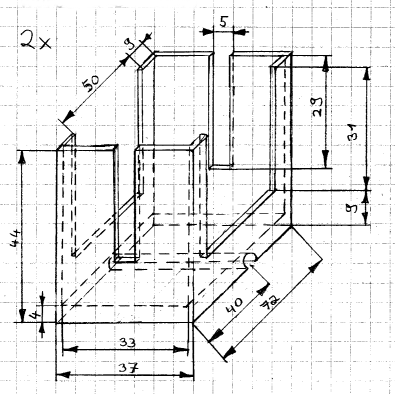
\includegraphics[width=6cm,angle=0]{content/pictures/motorenfuehrung.png}
\end{wrapfigure}
Eine Motorenführung weißt im Inneren eine effektive Länge von 68mm auf und erlaubt es uns somit je nach Größe der verwendeten Muttern die Motoren mit einer Länge von 40mm um ca. 15mm zu verstellen. Auf der hier gezeigten Skizze ist ein Schraubendurchmesser von 5mm vorgesehen. Dieser kann jedoch beliebig angepasst werden, wenn man die entsprechenden Maße der Motorenführung abändert. Durch eine Wandstärke von 2mm wird eine ausreichende Stabilität erreicht. Über den weiblichen Teil einer Steckverbindung am unteren Ende werden die Motorenführungen seitlich mit der weiter unten beschriebenen Bodenplatte verbunden.

\section{Motorenfassung}
Die beiden Motoren werden jeweils in einer Halterung eingefasst, welche später in den Motorenführungen beweglich gelagert sein werden, um die O-Ringe 
\begin{wrapfigure}[]{h}[4cm]{10cm}
	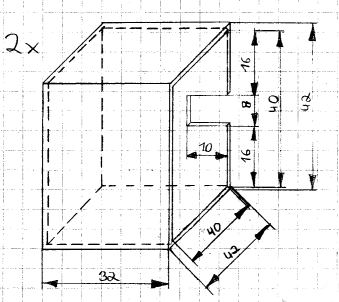
\includegraphics[width=6cm,angle=0]{content/pictures/motorenfassung.png}
\end{wrapfigure}
ein- und nachspannen zu können. Der Primärgrund für die Verwendung solcher Motorenfassungen ist jedoch der, dass die zu den Motoren gehörenden Treiberstufen über ein weiteres Bauteil an den Oberseiten der Motorenfassungen befestigt werden können. Auf diese Weise kann der für die Treiberstufen benötigte Platz auf der Bodenplatte eingespart werden. Zudem ist die Länge der Kabel zwischen Motor und Treiberstufe somit konstant. Um die Kabel, die seitlich aus den Motoren kommen zu berücksichtigen, befindet sich an einer Seite der Motorenfassungen eine entsprechende Aussparung.

\section{Treiberstufenhalteung}
Die Treiberstufenhalterung ist im Grunde lediglich eine quadratische Grundplatte mit einer Erhöhungen an jeder Ecke. Diese Erhöhungen dienen
\begin{wrapfigure}[]{h}[4cm]{10cm}
	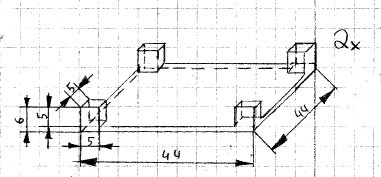
\includegraphics[width=6cm,angle=0]{content/pictures/treiberstufenhalterung.png}
\end{wrapfigure}
dazu, die Treiberstufen mit jeweils vier Schrauben an den Treiberstufenhalterungen befestigen zu können. Durch den Einsatz von Schrauben kommt hier ein Druck mit Wabenstruktur nicht in Frage. Deshalb werden die Treiberstufenhalterungen gefüllt gedruckt. Sie werden mit den Oberseiten der Motorenfassungen verklebt. 

\section{Vorderachsenhalterung}
Um die vorderen Räder an unserem Modell befestigen zu können, ist eine entsprechende Halterung notwendig. Die beiden Vorderräder sind 
\begin{wrapfigure}[]{h}[4cm]{10cm}
	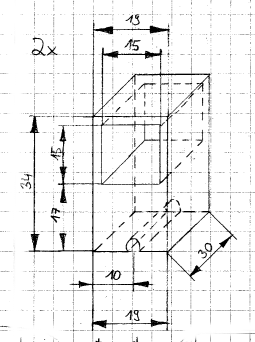
\includegraphics[width=6cm,angle=0]{content/pictures/vorderachsenhalterung.png}
\end{wrapfigure}
auf voneinander getrennten Achsen befestigt. Diese wiederum sind in jeweils einem Fischertechnik-Baustein frei drehbar gelagert. Um ein seitliches herausrutschen der Achsen zu verhindern werden an den Achsen befestigte Fischertechnik-Klemmen verwendet. Damit die Vorderräder auf dem selben Niveau wie die durch die relativ großen Schrittmotoren sehr hoch gelegenen Hinterräder sind, sind die Vorderachsenhalterungen 34mm hoch. Am oberen Ende befindet sich eine für die bereits zuvor genannten Fischertechnik-Bausteine vorgesehene Öffnung. Um eine ausreichende Stabilität gewährleisten zu können, ist auch hier eine Wandstärke von 2mm vorgesehen. Am unteren Ende befindet sich der weibliche Teil einer Steckverbindung, um die Vorderachsenhalterungen mit den auf der Bodenplatte befindlichen Gegenstücken zu verbinden.

\section{Bodenplatte}
Um ein funktionierendes Gesamtsystem zu erhalten, ist eine Bodenplatte von nöten. Auf ihr werden schließlich alle anderen Komponenten befestigt. Um keine Stabilität zu verlieren, wird sie aus einem einzigen Teil gedruckt. Die daraus resultierenden Nachteile, wie zum Beispiel die eingeschränkten Möglichkeiten durch den begrenzten Druckbereich des 3D-Druckers, mussten wir daher in Kauf nehmen.\\
Die Bodenplatte hat unter anderem aus Stabilitätsgründen eine Dicke von 5mm. Außerdem werden die anderen Bauteile über Steckverbindungen in abgesenkten Bereichen der Bodenplatte seitlich eingeschoben. Eine Breite von 105mm ergibt sich aus der breitesten Komponente, die auf der Bodenplatte befestigt werden muss, dem Akku. Die Länge von 214mm wurde durch den maximalen Druckbereich des von uns verwendeten 3D-Druckers bestimmt.\\
Jeweils vorne (auf der zugehörogen Skizze: unten) und hinten auf der Bodenplatte werden die Platinen mit den LEDs befestigt. Direkt hinter der vorderen LED-Platine finden sich jeweils links und rechts die Stellen, an denen die Vorderachsenhalterungen eingeschoben werden können. Dazwischen ist ein Durchbruch um die Kabel der vorderen LEDs nach unten durchführen zu können.\\ 
Im Bereich dahinter findet der für die Stromversorgung benötigte Akku seinen Platz. Durch die vier Durchbrücke können zwei Kabelbinder oder ähnliches gezogen werden, um den Akku an der Bodenplatte zu befestigen. Dahinter befindet sich eine oben geöffnete Box mit einem langen Durchbruch im inneren. Dort können die Kabel der Sensoren, welche an der Unterseite der Bodenplatte befestigt werden, und die Kabel der vorderen LEDs wieder nach oben geführt werden. So können sie einfach an dem direkt dahinter befestigten Raspberry Pi angeschlossen werden. Zu lange Kabel können dann in dieser Box verstaut werden.\\
Der RaspberryPi wird später an separat gedruckten Stelzen festgeschraubt, welche mit der Bodenplatte verklebt werden. Sie werden separat gedruckt, da auch diese Teile aufgrund der Tatsache, dass hier Schrauben zum Einsatz kommen, im Gegensatz zur Bodenplatte gefüllt gedruckt.\\
Die beiden darauffolgenden seitlichen Absenkungen mit den männlichen Teilen der Steckverbindungen dienen zur Befestigung der beiden Motorenführungen. Dazwischen ist wieder eine nach oben geöffnete Box, die zur Verkabelung dient. Diese ist zusätzlich teilweise nach vorne und komplett nach hinten geöffnet. So können auch bei der Verwendung eines Deckels Kabel nach vorne und hinten durchgeführt werden. Auch zum Anbringen der LED-Platine am hinteren Ende der Bodenplatte ist die Öffnung an der Hinterseite der Box aus Platzmangel notwendig. Am hintersten Bereich der Bodenplatte wird wie bereits oben beschrieben die Platine mit den Rücklichtern befestigt.
\begin{wrapfigure}[]{h}[4cm]{18.5cm}
	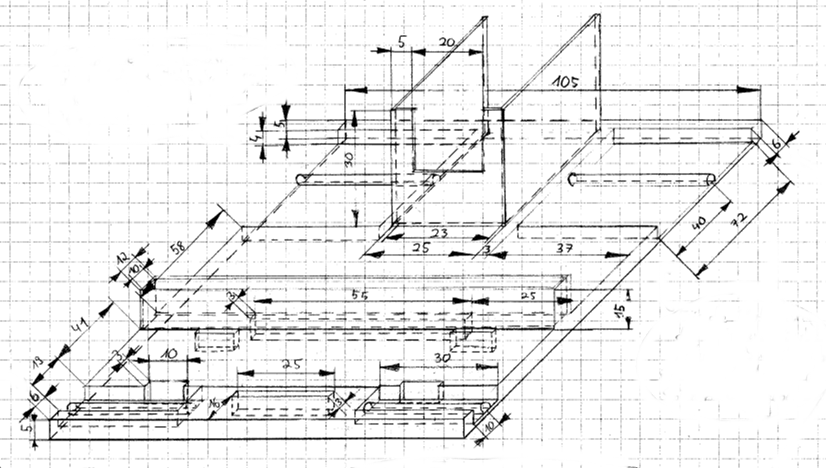
\includegraphics[width=14.5cm,angle=0]{content/pictures/bodenplatte.png}
\end{wrapfigure}

